%%%%%%%%%%%%%%%%%%%%%%%%%%%%%%%%%%%%%%%
%                                     %
%    Header Start                     %
%                                     %
%%%%%%%%%%%%%%%%%%%%%%%%%%%%%%%%%%%%%%%

% Din A 4 page with font size 12
%\documentclass[a4paper, twosides, 12pt]{article}
\documentclass[12pt,a4paper]{article}
\usepackage[english]{babel}
\usepackage[T1]{fontenc}
\usepackage[utf8]{inputenc}

%von niko
%\usepackage[margin=1.5in]{geometry}
%\usepackage{algorithmic}
%\usepackage{subcaption}
%\usepackage{lettrine}
%\usepackage[sc,osf]{mathpazo}
%\usepackage{booktabs}
% Es wird nicht eingerckt
\parindent=0mm

% arabic numbers for page numbering
\pagenumbering{roman}

% Definition der Ränder
\usepackage[paper=a4paper,left=30mm,right=30mm,top=25mm,bottom=25mm]{geometry}

% for declaring and using colors
\usepackage[table]{xcolor}
% define color values here
\definecolor{myblue}{rgb}{0.94, 0.97, 1.0}
\definecolor{Gray}{gray}{0.8}

% for apacite references
% \usepackage{apacite}
% \bibliographystyle{apacite}

% add references to Table of Contents
\usepackage[nottoc]{tocbibind}


% environment for definitions
\newtheorem{definition}{Definition}

\newtheorem{problem}[definition]{Problem}

% enumerate change
\usepackage{paralist}

% for romanic numbers
\newcommand{\RM}[1]{\MakeUppercase{\romannumeral #1{}}}

% for inserting graphics
\usepackage{graphicx}
\usepackage{subfigure}
\usepackage{tikz}
\usetikzlibrary{arrows,shapes,positioning,shadows,trees}
\tikzset{
  basic/.style  = {draw, text width=3cm, drop shadow, font=\sffamily, rectangle},
  root/.style   = {basic, rounded corners=2pt, thin, align=center,
                   fill=green!30},
  level 2/.style = {basic, rounded corners=6pt, thin,align=center, fill=green!60,
                   text width=8em},                                                  
  level 3/.style = {basic, thin, align=left, fill=blue!60, text width=6.9em}
}
\usepackage{wrapfig}

%\usepackage{pstricks}

% for inserting tables
\usepackage{tabularx, multirow, array, dcolumn}

% for mathematical symbols
\usepackage{amsmath}
\usepackage{amssymb}
\usepackage{latexsym}

% for graphics
\usepackage{tikz}
\usetikzlibrary{arrows,positioning}
\usepackage{color}

%for ipa
\usepackage{tipa}

% pdf LaTeX for linguistic examples
\usepackage{linguex}

%%for OT tables
\usepackage{pifont}    %for pointing hand
\usepackage{arydshln}    %for dashed lines
\usepackage{rotating}    %for angled text

% for inserting pdfs
\usepackage{pdfpages} 

% for inserting trees
\usepackage{qtree}
%\usepackage{ps-trees}

% for line distance
\usepackage{setspace}

% for thick lines
\usepackage{booktabs}

% for footer and header
\usepackage{fancyhdr}

%resizing
\usepackage{adjustbox}

% landscape format
\usepackage{lscape}
% for caption formatting
\usepackage{caption}

% for quotation marks
\newcommand{\Gu}{\glqq{}}		% quotation marks top
\newcommand{\Go}{\grqq\xspace} 	% quotation marks bottom
\newcommand{\Ga}{\textquotedblleft{}} % american quotation marks top start
\newcommand{\Ge}{\textquotedblright\xspace} % american quotation marks top end
\newcommand{\Tg}[1]{\textsubscript{#1}}		% lower
\newcommand{\Hg}[1]{\textsuperscript{#1}}	% higher
\newcommand{\leer}{\vspace*{\baselineskip}}% empty line

% reference with \tab, \fig, \sec to tables, graphics, and paragraphs
\usepackage{titleref}
\usepackage{prettyref}
\newrefformat{tab}{siehe Tab. \ref{#1} "\titleref{#1}" auf der Seite \pageref{#1}}% tables
\newrefformat{fig}{siehe Fig. \ref{#1} "\titleref{#1}" auf der Seite \pageref{#1}}% graphics
\newrefformat{sec}{siehe Abschnitt \ref{#1} "\titleref{#1}" auf der Seite \pageref{#1}}% paragraphs
%\pageref{#1}

%changes the numbering of figure and table
\numberwithin{figure}{section}
\numberwithin{table}{section}
\numberwithin{definition}{section}

% heading tweaks
\usepackage{titlesec}
\titleformat{\section}
{\normalfont\Large\bfseries}
{\thesection}
{1em}
{}
\titleformat{\subsection}
{\normalfont\Large\bfseries}
{\thesubsection}
{1em}
{}
\titleformat{\subsubsection}
{\normalfont\Large\bfseries}
{\thesubsubsection}
{1em}
{}

\newcommand{\HRule}{\rule{\linewidth}{0.5mm}}

% global scaling of table size
\usepackage{etoolbox}

\AtBeginEnvironment{tabular}{\scriptsize}
\AtBeginEnvironment{tabularx}{\scriptsize}

% Bibliography
\usepackage[style=authoryear,backend=biber]{biblatex}
\addbibresource{bibliography.bib}

%%%%%%%%%%%%%%%%%%%%%%%%%%%%%
%                           %
%      Document Start       %
%                           %
%%%%%%%%%%%%%%%%%%%%%%%%%%%%%
\begin{document}
\begin{titlepage}
\begin{center}


% Upper part of the page. The '~' is needed because \\
% only works if a paragraph has started.
%\\textsc{includegraphics[width=0.68\textwidth]{bilder/unilogo.png}~\\[1.5cm]
%~\\[1.5cm]
%\vspace{-1.0cm}}

\textsc{\LARGE Master's Thesis}\\[0.8cm]

\textsc{\large in Computational Linguistics}\\[0.5cm]

% Title
\HRule \\[0.4cm]
{  \bfseries \fontsize{22}{37} \selectfont Deconstructing Constructed Languages}\\
\vspace{0.4em}

\HRule \\[1.5cm]



% Author and supervisor
\begin{minipage}{0.4\textwidth}
\begin{flushleft} \large
\emph{Author:}\\
Connor \textsc{Kirberger}
\end{flushleft}
\end{minipage}
\begin{minipage}{0.5\textwidth}
\begin{flushright} \large
%\emph{1st Examiner \& Supervisor:} \\
\emph{Supervisors:} \\
Çağrı \textsc{Çöltekin} \\
Christian \textsc{Bentz}\\
\end{flushright}
\end{minipage}


\vfill



\textsc{\large Seminar f\"ur Sprachwissenschaft\\Eberhard-Karls-Universit\"at T\"ubingen}\\[1.5cm]



% Bottom of the page
{\large December 2023}

\end{center}
\end{titlepage}


%---------------------
% Ende der Titelseite
%---------------------

%----------------------------
% Selbstständigkeitserklrung
%----------------------------

\noindent

Hiermit versichere ich, dass ich die Arbeit selbständig verfasst, keine anderen als die angegebenen Hilfsmittel und Quellen benutzt, alle wörtlich oder sinngemäß aus anderen Werken übernommenen Aussagen als solche gekennzeichnet habe und dass die Arbeit weder vollständig noch in wesentlichen Teilen Gegenstand eines anderen Prüfungsverfahrens gewesen ist und dass die Arbeit weder vollständig noch in wesentlichen Teilen bereits veröffentlicht wurde sowie dass das in Dateiform eingereichte Exemplar mit den eingereichten gebundenen Exemplaren übereinstimmt.\\[4em]
I hereby declare that this paper is the result of my own independent scholarly work.
I have acknowledged all the other authors' ideas and referenced direct quotations
from their work (in the form of books, articles, essays, dissertations, and on the
internet). No material other than that listed has been used.
\\[18mm]
T\"ubingen, \today \hspace{6.0cm} \\%[10mm]\\
\begin{flushright}

\rule{0.4\textwidth}{0.2pt}\\
Firstname Surname
\end{flushright}
\pagestyle{empty}
\newpage

% inserting official anti-plagiarism statement
% \includepdf{antiplagiatserklaerung.pdf}
\newpage
%------------
% Textanfang
%------------

%% Inhaltsverzeichnis
\tableofcontents
\thispagestyle{empty}
%% Anderthalbzeiliger Zeilenabstand ab hier
\onehalfspacing
%\singlespacing

%% Keine Seitenzahl
\pagestyle{empty}

%% Beginn einer neuen Seite
\newpage

%% Abstract
\abstract{

Write the abstract here.
}
\newpage

%% Beginn einer neuen Seite
%\newpage

%%list of figures
\listoffigures
% list of tables
\listoftables


% list of abbreviations
\section*{List of Abbreviations}
\addcontentsline{toc}{section}{List of Abbreviations}

\begin{tabular}{lcl}
\textbf{NLP} & ~~~ & Natural Language Processing \\
\textbf{PCA} & ~~~ & Principle Component Analysis \\
\textbf{TF-IDF} & ~~~ & Term Frequency - Inverse Document Frequency \\
\textbf{RNN} & ~~~ & Recurrent Neural Network \\
\textbf{LSTM} & ~~~ & Long Short-Term Memory \\
\textbf{SVM} & ~~~ & Support Vector Machine \\
\textbf{XML} & ~~~ & eXtensible Markup Language \\
\textbf{TTR} & ~~~ & Type-Token Ratio \\
\textbf{MATTR} & ~~~ & Moving-Average Type-Token Ratio \\

\end{tabular}
\newpage

%\listoftables
%\newpage

%% header with section heading and right-aligned page number
\pagestyle{fancy}
\fancyhf{}
\fancyhead[L]{\textcolor{gray}{\slshape\nouppercase{\rightmark}}}
\fancyhead[R]{\thepage}
\fancyfoot[R]{\textcolor{gray}{Seminar für Sprachwissenschaft Universität Tübingen}}
\renewcommand{\headrulewidth}{0.4pt}

\renewcommand{\headrulewidth}{0.5pt}
\renewcommand{\footrulewidth}{0.5pt}



%--------
% TEXT
%--------
% page numbers start with 1 here.
\setcounter{page}{1}
\pagenumbering{arabic}

\section{Introduction} 
\label{sec:intro}

Constructed languages---also called artificial languages, invented languages, planned languages, glossopoeia, or more simply as "conlangs", a shortened neologism derived from combining the beginning letters of "constructed" and "language" \parencite{douglas2015book}---are languages that are consciously and purposefully created for some intended use, usually being defined in antithesis to the spontaneous and organic method in which natural languages arise and develop \parencite{sanders2016article}. Despite this distinction in common definition, however, the separation between natural and constructed language might not always be so clear when analyzed in greater detail \parencite{goodall2022article}. 

The aforementioned intended uses for constructed languages can range broadly. Some are created specifically for fictional media, often seen in the genres of fantasy or science-fiction, with some more well-known examples being J. R. R. Tolkien's Elvish languages (Quenya, Sindarin, Nandorin, etc.) found in the world of Middle-earth in his novels, Marc Okrand's Klingon language from the Star Trek universe, and David J. Peter's Dothraki language used in George R. R. Martin's A Song of Ice and Fire novels along with their television adaptation, Game of Thrones \parencite{punske2020book}. Others are created to function as international auxiliary languages, the most famous example (based on estimated number of speakers) arguably being Esperanto, created in the 19\textsuperscript{th} Century by L. L. Zamenhof. Typically, constructed languages can be further distinguished and categorized based on their various purposes for being created.

\subsection{Motivation}
\label{ssec:motivation}

% Initially, I began my research with the intention of formulating an approach for deciphering the Voynich Manuscript, an illustrated folio containing handwritten text from a still---at the time of writing this at least---unknown language and in an unknown script or cipher. One theory, as noted by \textcite{Reddy2011paper}, is that the underlying language may not be natural.

\subsection{Scope of Study \& Research Question}
\label{ssec:scope}

As previously noted, the specific boundaries which separate constructed from natural languages are not always clearly or consistently defined---even amongst linguists. 

This study analyzes the linguistic features of constructed and natural languages and seeks to make a comparison on the differences, if any exist, between the two. Because of the wide-ranging nature of conducting such a broad analysis, there will of course be many features left unconsidered. With this in mind and following the precedent set by other related research on this topic, the focus in this particular study is mainly on features such as entropy, morphological complexity, and lexical diversity of each language, based on the corpora used. Ultimately, I seek to contribute to answering the age-old question of what defines a language.

The following is a breakdown of the structure of this thesis from here onward: the next section provides relevant background information, including an overview on constructed languages and a comprehensive review of related literature that examines the prior theoretical groundwork laid for exploring linguistic similarities and differences between constructed and natural languages; section \ref{sec:methodology} covers in detail the methodology taken in this research, from an explanation of the data used to the various experiments performed; section \ref{sec:results} presents the results of the study and discussion of these follows in section \ref{sec:discussion}; lastly, section \ref{sec:conclusion} consists of a conclusion as well as elaboration for possible future work.

\section{Background}
\label{sec:background}

The vast landscape of linguistic research comprises a myriad of studies delving into the intricacies of languages, both natural and constructed. This section will begin with a brief examination into constructed languages, defining what they are as well as their various purposes, as this is crucial to the study. 

Finally, I will discuss the various computational methods implemented and provide some background information on how they work. 

\subsection{Constructed Languages}
\label{ssec:conlangs}

Constructed languages are actually a broad category of languages comprised of several sub-genres, differentiated according to their intended purpose for being created. These include philosophical languages, international auxiliary languages, 

\subsection{Prior Studies}
\label{ssec:priorstudies}



\subsection{Computational Methods}
\label{ssec:computationalmethods}

\section{Methodology}
\label{sec:methodology}

In this section, I explain in greater detail the materials and dataset used, as well as the approaches and steps taken to arrive at my results. Because of the broad nature of this study, several different experiments are done to test various linguistic features. Namely, these features are morphological complexity, character and word frequency distributions, and character entropy. Once these were calculated for each language, the task became that of classification through the use of 2 classifier models: outlier detection and a decision tree. 

\subsection{Data}
\label{ssec:data}

In total, twenty-two languages are analyzed in this study. Four of these are constructed languages: Esperanto, Interlingua, Lingua Franca Nova, and Ido. The remaining eighteen are natural languages: German, English, Spanish, Polish, Vietnamese, Indonesian, Turkish, Tagalog, Hungarian, French, Finnish, Italian, Dutch, Occitan, Danish, Swedish, Afrikaans, and Icelandic. 

To briefly introduce the constructed languages used here, Esperanto is the most widely spoken constructed language

As this study is cross-linguistic in nature, it would naturally be ideal to use parallel corpora, as this would enable more conclusive comparative analysis. However, creating or finding parallel corpora that also includes the aforementioned constructed languages is rather challenging due to the limited availability of resources for many of them. Therefore, I instead opted for a more practical approach of using 

\subsubsection{Wikimedia}
\label{ssec:wikimedia}

Text data was collected from Wikimedia database dumps---large files containing Wikipedia articles for a given language which are formatted in XML. The corpus sizes were constricted to be comparable in length based on number of words, while still maintaining complete sentences. The smallest corpus came from Lingua Franca Nova, so its size was the minimum value used to shorten the others. 

\subsection{Data Preprocessing}
\label{ssec:datapreprocessing}

Preprocessing text data is essential for NLP tasks. As this study covers a broad range of different languages and includes constructed languages, which often have less resources available, meticulous effort was made to obtain as close to a parallel set of corpora as possible and to clean the text thoroughly. 

After extracting the text from the dump files through the use of a Python script\footnote{https://github.com/apertium/WikiExtractor/tree/master}, regular expressions were used to remove page titles, links, headers, fragments, and other extraneous symbols. The text was then made all lowercase and split by the periods---while also attempting to account for abbreviations---to make separate sentences, and all characters that were not part of the language's writing system were removed in an attempt to have only that language's words, without any foreign words that occasionally appear in the scraped Wikipedia texts. Remaining punctuation and numbers were also removed. The end result was a single corpus file corresponding to each language, with each line of the files being a single sentence. 

\subsection{Feature Extraction}
\label{ssec:featureextraction}

Once the data had been preprocessed, some initial values were calculated to be used as a starting point for our investigation in comparing natural and constructed languages. These were Zipf's law of abbreviation, type-token ratio (TTR), moving-average type-token ratio (MATTR), and character and word distribution entropies.

\subsubsection{Type-Token Ratio}
\label{ssec:ttr}

TTR is a way of measuring lexical diversity. It is calculated using the following formula: \[TTR = \frac{\sum_{i=1}^{n}\delta(w_i)}{n}\]

\subsubsection{Moving-Average Type-Token Ratio}
\label{ssec:mattr}

A glaring issue with TTR, however, is that it can vary widely based on a text's length. The longer a particular text, the higher the likelihood of repetition occurring. There have been several solutions proposed to address this issue, one being MATTR. MATTR is given in the formula \[MATTR_i = \frac{TTR_1+TTR_2+...+TTR_i}{i}\]

\subsubsection{Entropy}
\label{ssec:entropy}

In information science, entropy means... 
In linguistics, entropy refers to...

The entropy was calculated for the character and word distributions in each of the corpora, given by the following formula: \[H = -\sum_{i=1}^{n}p_{i}\log_{2}p_{i}\]

\begin{figure}
  \centering
        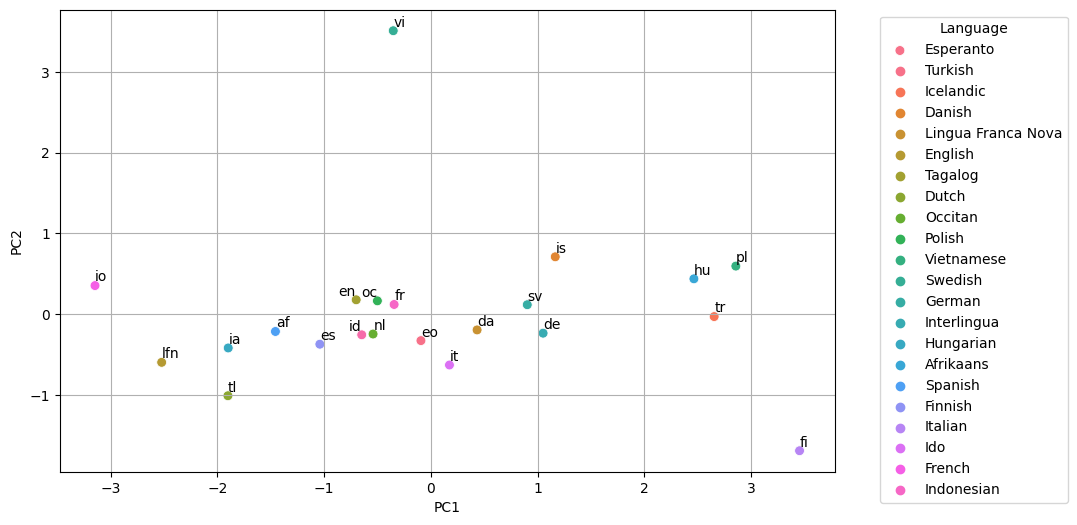
\includegraphics[width=1.0\textwidth]{pcaanalysis.png}
        \caption{Principal Component Analysis on TTR, MATTR, Word and Char Distribution Entropy}
        \label{fig:pcaanalysis}
\end{figure}

\subsubsection{Morphological Complexity}
\label{ssec:morphologicalcomplexity}

The morphological systems of each language was also investigated and analyzed, specifically their complexities. Morfessor, 

\subsubsection{Perplexity}
\label{ssec:perplexity}

One measure used for evaluating and comparing the similarities and differences between natural and constructed languages is that of entropy. Specifically, the entropy of 

\subsubsection{PCA}
\label{ssec:pca}

Principal Component Analysis was performed for dimensionality reduction. 

A script was used to increase readability of the text in the graph\footnote{https://github.com/Phlya/adjustText}.

\subsection{Classification Models}
\label{ssec:classification}

\subsubsection{Decision Tree}
\label{ssec:decisiontree}

Decision Tree Classifier...

\begin{figure}
  \centering
        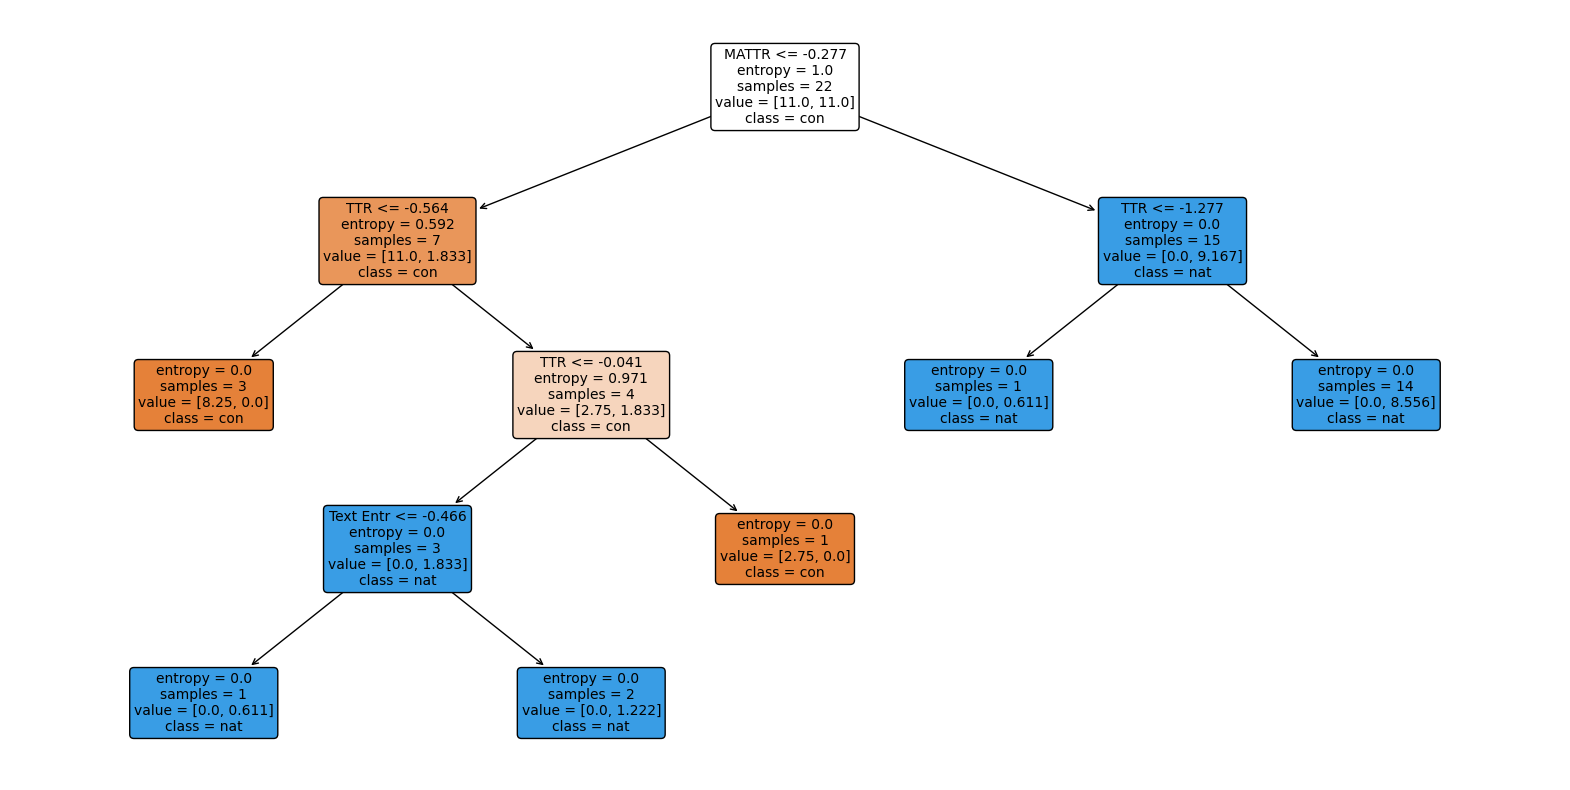
\includegraphics[width=1.0\textwidth]{decisiontree.png}
        \caption{Decision Tree Classifier}
        \label{fig:decisiontree}
\end{figure}

\subsubsection{Outlier Detection}
\label{ssec:outlierdetection}

\section{Results}
\label{sec:results}

In this section

\section{Discussion}
\label{sec:discussion}

\section{Conclusion}
\label{sec:conclusion}

\subsection{Future Work}
\label{ssec:futurework}

The research presented in this thesis is far from encompassing all there is to the topic of defining language, and distinguishing between constructed and natural language. At present, this is an area of research with ample room for potential development. 

Limiting factors: number of languages and which languages/language families, lack of real parallel corpora, problems associated with low-resource languages, relatively narrow scope of experimentation,

\newpage
\section{Acknowledgments}
\label{sec:acknowledgments}
I would like to thank ....

\newpage
\printbibliography

\end{document}

